\documentclass[UTF8]{report}
\usepackage{graphicx}
\usepackage{xetexko}

\title{%
    <컴퓨터프로그래밍 3> 실습 보고서 \\ 
    \large [제 03 주] 마방진}
\author{201704150 허강준}
\date{\today}


\begin{document}
    \maketitle
    \tableofcontents

    \chapter{프로그램 설명서}
        본 보고서에서는 마방진에 대한 객체를 정의하고 처리하는 프로그램에 대해 기술한다.

        \section{프로그램의 전체 설계 구조 (MVC 등)}
            
            \paragraph{%
                \normalfont 1, 2주차에서 사용했던 기존의 프레임워크를 재활용하며, 마방진 계산의 처리를 위해 \texttt{MagicSquare} 모듈을 도입하였다. 최대 처리 가능 크기(\texttt{MAX\_ORDER})를 도입하도록 한 것에 따라, Visual Studio에서 설정한 기본 스택 사이즈인 16KB를 넘을 수 있으므로 부득이하게 Heap에 마방진 객체를 할당하였다.
            }

            \paragraph{%
                \normalfont 마방진을 표현하기 위한 구조체를 \texttt{App\_Start} 에 지역번수로서 선언하지 않은 이유는 위에서 언급한 스택 사이즈의 문제이며 이는 프로젝트 설정 등을 통하여 해결할 수 있으나 채점 과정에서 문제가 될 수 있으므로 정석을 따르도록 한다.
            }
            
        \section{함수 설명서}

            \paragraph{\texttt{MagicSquare\_create(unsigned int order)}}
            \paragraph{%
                \normalfont 새 MagicSquare 객체를 생성한다.
            }

            \paragraph{\texttt{MagicSquare\_destroy(MagicSquare* \_this)}}
            \paragraph{%
                \normalfont \texttt{MagicSquare\_create(unsigned int order)} 로 생성한 마방진을 제거하고 할당된 메모리를 해제한다.
            }

            \paragraph{\texttt{MagicSquare\_orderIsValid(int order)}}
            \paragraph{%
                \normalfont 마방진의 차수는 3 이상의 홀수에 대해서, 그리고 99로 정의된 최대 차수보다 작아야 한다. 따라서 이 조건을 만족하지 못할 경우 \texttt{false}를 리턴한다.
            }

            \paragraph{\texttt{MagicSquare\_clear(MagicSquare* \_this)}}
            \paragraph{%
                \normalfont 마방진 풀이 프로그램은 프로그램이 종료될 때 까지 반복할 수 있으므로, 기존에 남아있는 마방진 데이터를 삭제한다.
            }

            \paragraph{\texttt{MagicSquare\_solve(MagicSquare* \_this)}}
            \paragraph{%
                \normalfont 실습 자료에서 제시한 알고리즘에 따라 마방진을 풀이한다. 객체를 사용하지 않으므로 풀이할 차수를 인자로 제공한다.
            }

        \section{종합 설명서}

            \paragraph{%
                \normalfont 마방진은 모든 행과 열, 그리고 대각선의 합이 전부 동일하도록 수를 정사각행렬에 배치한 것이다. 1부터 $n^2$ 까지의 자연수가 차례로 배치된다.첫번째 행의 중앙부터 
            }

            \paragraph{%
                \normalfont 본 프로그램에서는 실습 자료에서 제시된 알고리즘을 사용하였으며 그 방법은 다음과 같다:
            }

            \begin{itemize}
                \item 첫번째 행의 중앙 열 s부터 시작한다. (차수 n에 대해 $s = n >> 1$, >>는 우측 쉬프트 연산)
                \item 오른쪽 위로 올라가며 1씩 증가한다.
                \item 만일 채우고자 하는 칸에 이미 값이 채워진 경우 현재 칸의 바로 아래 칸을 채운다.
                \item 이때 행렬을 벗어날 경우, 다음 규칙에 따라 다음 칸을 선정한다:\\
                      \begin{itemize}
                          \item 위쪽 방향일 경우 마지막 행으로 이동한다.
                          \item 아랫쪽 방향일 경우 처음 행으로 이동한다.
                          \item 오른쪽 방향일 경우 첫 열로 이동한다.
                          \item 왼쪽 방향일 경우 마지막 열로 이동한다.
                      \end{itemize}
            \end{itemize}
            
    \chapter{프로그램 장단점/특이점 분석}
        \section{\_this?}
            \paragraph{%\
                \normalfont 대부분의 객체지향 프로그래밍 언어들은 자기 자신을 지칭하는 예약어를 언어 스펙에서 제공한다. C++/Java의 \texttt{this} 가 그 경우이며 이 외에도 \texttt{self}(Javascript, Python), \texttt{Me}(Visual Basic) 등이 있다.
            }

            \paragraph{%\
                \normalfont 이들 키워드는 대개 해당 클래스/구조체의 레퍼런스로 구현되나, C에서는 객체지향에 대해 이러한 언어적 지원이 전무하므로 메서드로 사용될 함수를 호출할 때 첫번째 인자로 해당 객체의 포인터를 전달해주도록 한다.
            }

            \paragraph{%\
                \normalfont 따라서 C의 경우 \texttt{this}를 사용할 수 있으나, Visual Studio의 \texttt{this}는 MSVC에서 사용중인 예약어이므로 컴파일 오류가 발생하며 에디터에서도 하이라이팅되어 코드 가독성에 혼란을 줄 여지가 있다. 따라서 본 강의 내내 진행되는 프로젝트에서는 \texttt{\_this}를 사용하도록 한다.
            }            

        
    \chapter{실행 결과 분석}
        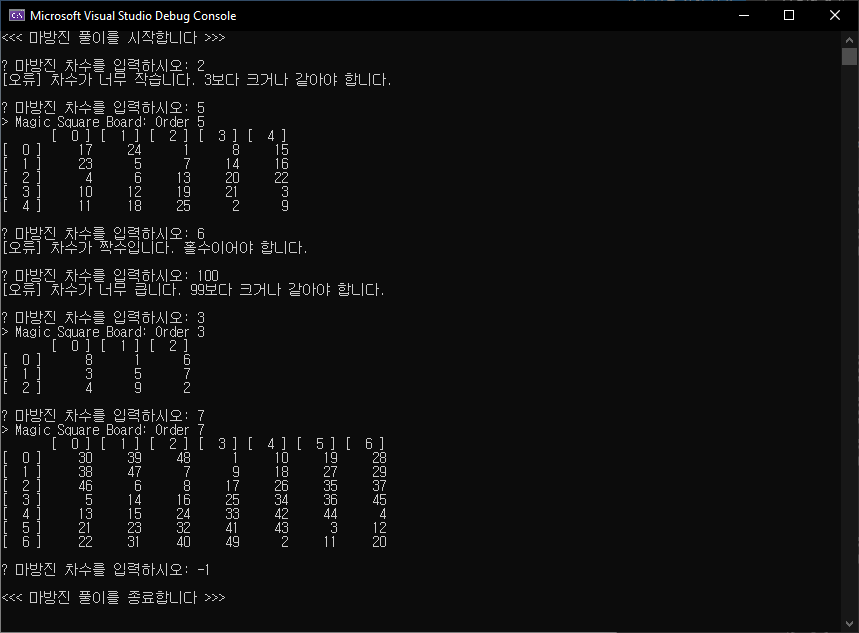
\includegraphics[width=\textwidth]{test_result.png}
        \section{입력과 출력}
            실습 자료에서 제시된 입력을 사용하였으며 모든 경우에 대해 정상적으로 처리됨을 확인하였음.
        \section{결과 분석}
            실습 자료에서 제시된 출력과 동일함을 확인하였음.

    \chapter{소스코드}
        소스코드는 제출된 압축파일에 같이 동봉되어있으며 GitHub (0x00000FF/CNUCSE-Computer-Programming-III-2020-Spring) 에서도 열람할 수 있다.
\end{document}